\documentclass[aspectratio=169, table]{beamer}

\usepackage[utf8]{inputenc}
\usepackage{listings} 

\usetheme{Pradita}

\subtitle{IF140303-Web Application Development}

\title{Session-06:\\
\Huge{
Avatar Generator 2/2\\
\vspace{5pt}
}
}
\date[Serial]{\scriptsize{PRU/SPMI/FR-BM-18/0222}}
\author[Pradita]{\small{\textbf{Alfa Yohannis}}}

\lstdefinelanguage{Elixir} {
	keywords={case, def, defmodule, do, end, for, if, else, true, false},
	basicstyle=\ttfamily\small,
	keywordstyle=\color{blue}\bfseries,
	ndkeywords={@moduledoc, iex, Enum, @doc},
	ndkeywordstyle=\color{purple}\bfseries,
	sensitive=true,
	numbers=left,
	numberstyle=\tiny\color{gray},
	breaklines=true,
	frame=lines,
	backgroundcolor=\color{lightgray!10},
	tabsize=2,
	comment=[l]{\#},
	morecomment=[s]{/*}{*/},
	commentstyle=\color{gray}\ttfamily,
	showstringspaces=false,
	% string settings
	morestring=[b]",
	morestring=[b]',
	stringstyle=\color{black}\ttfamily, % default, will be overridden
	moredelim=[s][\color{blue}\ttfamily]{"}{"},   % double quotes
	moredelim=[s][\color{teal}\ttfamily]{'}{'}    % single quotes
}


\lstdefinelanguage{bash} {
	keywords={},
	basicstyle=\ttfamily\small,
	keywordstyle=\color{blue}\bfseries,
	ndkeywords={iex},
	ndkeywordstyle=\color{purple}\bfseries,
	sensitive=true,
	commentstyle=\color{gray},
	stringstyle=\color{red},
	numbers=left,
	numberstyle=\tiny\color{gray},
	breaklines=true,
	frame=lines,
	backgroundcolor=\color{lightgray!10},
	tabsize=2,
	comment=[l]{\#},
	morecomment=[s]{/*}{*/},
	commentstyle=\color{gray}\ttfamily,
	stringstyle=\color{purple}\ttfamily,
	showstringspaces=false
}

\begin{document}
	
	\frame{\titlepage}
	
		\begin{frame}[fragile]
		\frametitle{Contents}
		\vspace{20pt}
		\begin{columns}[t]
			\column{0.5\textwidth}
			\tableofcontents[sections={1-6}]
			
			\column{0.5\textwidth}
			\tableofcontents[sections={7-99}]
		\end{columns}
	\end{frame}


\section{Introduction}

\begin{frame}[fragile]{Introduction}
\vspace{20pt}
This section explains the development of an \textbf{avatar generator} built using the Elixir programming language.  
The program showcases key Elixir features:
\begin{itemize}
  \item \texttt{defstruct} for defining structured data types,
  \item \texttt{defmodule} for modular organization,
  \item \texttt{Application} behavior for managing runtime lifecycle.
\end{itemize}

\textbf{The generator} takes a text input (e.g., a username) and computes its \textbf{MD5 hash}, which is a \textbf{128-bit} (\textbf{16-byte}) fixed-length value.  
\textbf{Each byte} is \textbf{converted} into an \textbf{integer }between \textbf{0 and 255}, forming a sequence of numbers that represents the hash in numeric form.  
These integers are then used to:
\begin{itemize}
  \item determine which grid cells will be filled,
  \item assign colors or symmetry patterns to each region.
\end{itemize}
Thus, every unique input string produces a distinct yet deterministic avatar.
\end{frame}


\subsection{Avatar Generator}
\begin{frame}[fragile]{Avatar Generator}
\begin{figure}
  \centering
  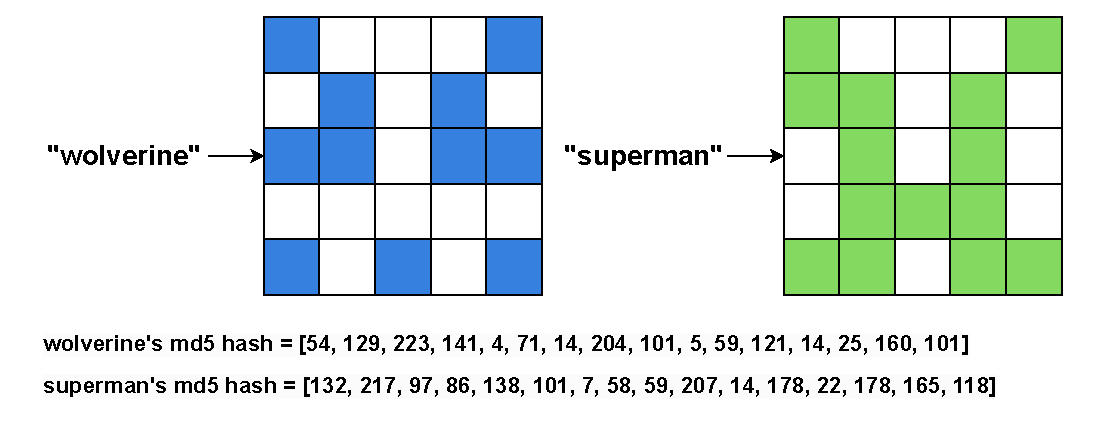
\includegraphics[width=\linewidth]{../../assets/avatar-example.pdf}
\end{figure}
\vspace{-10pt}
The 128-bit MD5 hash is split into 16 integers (0–255), each encoding color or grid placement.  
These values define the avatar’s pattern and symmetry, ensuring every input yields a unique, consistent design.


\end{frame}

\subsection{Avatar Pipeline}

\begin{frame}[fragile]{Avatar Pipeline}
\begin{figure}
  \centering
  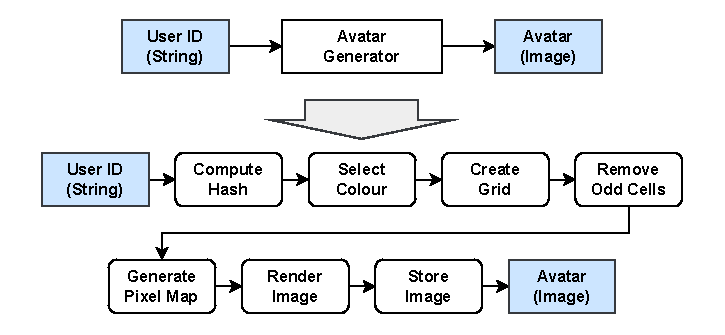
\includegraphics[width=.88\linewidth]{../../assets/avatar-pipeline.pdf}
\end{figure}
Input text is hashed (MD5, 128-bit/16 bytes) and drives color and layout. Functions run sequentially to transform data into a rendered PNG image.
\end{frame}

\begin{frame}[fragile]{Pipeline Code}
\vspace{20pt}
\begin{lstlisting}[language=Elixir]
compute_hash
|> select_color
|> create_grid
|> remove_odd_cells
|> generate_pixel_map
|> render_image
|> store_image
\end{lstlisting}

\small
\textbf{compute\_hash}: MD5 → 16 integers (0–255).  
\textbf{select\_color}: derives RGB from first bytes.  
\textbf{create\_grid}: builds 5×5 layout with symmetry.  
\textbf{remove\_odd\_cells}: keep even-valued cells.  
\textbf{generate\_pixel\_map}: map cells to coordinates.  
\textbf{render\_image}/\textbf{store\_image}: draw and save PNG.
\end{frame}

\subsection{Avatar Computation}

\begin{frame}[fragile]{Avatar Computation}
\begin{columns}[T,totalwidth=\textwidth]
  \begin{column}{0.4\textwidth}
    \small
    \begin{itemize}
      \item The avatar is generated as a \textbf{5×5 grid} image.
      \item \textbf{Columns 4 and 5 mirror columns 2 and 1}, creating symmetry and visual balance.
      \item \textbf{The first three columns} use integer values of the MD5 hash of the \texttt{username}.
      \item \textbf{Even} values fill colored cells; \textbf{odd} values remain white.
      \item \textbf{The first three hash bytes} define the RGB color used for the avatar.
    \end{itemize}
  \end{column}
\hfill
  \begin{column}{0.6\textwidth}
    \centering
    \begin{figure}
      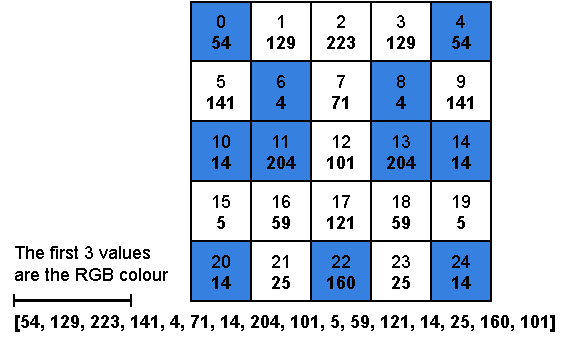
\includegraphics[width=\linewidth]{../../assets/avatar-computation.pdf}
      \caption{Hash integers, mirroring, and RGB mapping.}
    \end{figure}
  \end{column}
\end{columns}
\end{frame}

\section{Filtering Cells: \texttt{remove\_odd\_cells/1}}

\begin{frame}[fragile]{Filtering Cells: \texttt{remove\_odd\_cells/1}}
\vspace{20pt}
\small
The \texttt{remove\_odd\_cells/1} function filters the avatar grid to retain only even-valued cells.  
It helps simplify the final pattern and maintain symmetry.  

\begin{itemize}
  \item Uses \texttt{Enum.filter/2} to traverse each grid cell.
  \item Keeps only cells where \texttt{rem(code, 2) == 0}.
  \item Removes odd-numbered cells that do not meet the condition.
  \item Produces a cleaner, even-coded grid for rendering.
\end{itemize}

\begin{lstlisting}[language=Elixir]
def remove_odd_cells(%Avatar.Image{grid: grid} = image) do
  grid = Enum.filter grid, fn({code, _index}) ->
    rem(code, 2) == 0
  end
end
\end{lstlisting}
\end{frame}

\section{Generate Pixel Map: \texttt{generate\_pixel\_map/1}}

\begin{frame}[fragile]{Generate Pixel Map: \texttt{generate\_pixel\_map/1}}
\vspace{20pt}
\small
The \texttt{generate\_pixel\_map/1} function converts the filtered grid into a pixel map that defines  
the exact coordinates of each cell on the image canvas. It calculates the \texttt{x} and \texttt{y}  
positions based on each cell index, determines the \texttt{top\_left} and \texttt{bottom\_right}  
points for 50×50 pixel blocks, and stores the resulting coordinate pairs in the \texttt{pixel\_map} field.

\begin{lstlisting}[language=Elixir, basicstyle=\ttfamily\scriptsize]
def generate_pixel_map(%Avatar.Image{grid: grid} = image) do
  pixel_map = Enum.map grid, fn({_code, index}) ->
    x = rem(index, 5) * 50
    y = div(index, 5) * 50

    top_left = {x, y}
    bottom_right = {x + 50, y + 50}

    {top_left, bottom_right}
  end

  %Avatar.Image{image | pixel_map: pixel_map}
end
\end{lstlisting}
\end{frame}


\section{Rendering Image: \texttt{render\_image/1}}


\begin{frame}[fragile]{Rendering Image: \texttt{render\_image/1}}
\vspace{20pt}
\small
The \texttt{render\_image/1} function generates the final avatar image from the pixel map and color data.  
It uses the Erlang \texttt{:egd} module to create a 250×250 canvas, apply the selected RGB color,  
and draw filled rectangles for each cell in the pixel map before rendering the complete image.

\begin{lstlisting}[language=Elixir, basicstyle=\ttfamily\scriptsize]
def render_image(%Avatar.Image{color: color, pixel_map: pixel_map}) do
  image = :egd.create(250, 250)
  fill = :egd.color(color)

  Enum.each pixel_map, fn({start, stop}) ->
    :egd.filledRectangle(image, start, stop, fill)
  end

  :egd.render(image)
end
\end{lstlisting}
\end{frame}

\section{Storing Image: \texttt{store\_image/2}}

\begin{frame}[fragile]{Storing Image: \texttt{store\_image/2}}
\vspace{20pt}
\small
The \texttt{store\_image/2} function saves the rendered image as a \texttt{.png} file.  
It takes two arguments — the image binary and the original \texttt{input} string — which is used to name the output file.  
The built-in \texttt{File} module writes the binary image data directly to disk.

\begin{lstlisting}[language=Elixir, basicstyle=\ttfamily\scriptsize]
def store_image(image, input) do
  File.write("#{input}_avatar.png", image)
end
\end{lstlisting}
\end{frame}

\section{Project Configuration: \texttt{mix.exs}}

\begin{frame}[fragile]{Project Configuration: \texttt{mix.exs}}
\vspace{20pt}
\small
The \texttt{mix.exs} file defines essential project settings in the \texttt{AvatarGenerator.MixProject} module.  
It contains metadata, dependencies, and application configuration generated automatically by \texttt{mix new}.  
The module uses \texttt{Mix.Project} to manage build, compile, and dependency tasks for the Elixir project.

\begin{lstlisting}[language=Elixir, basicstyle=\ttfamily\scriptsize]
defmodule AvatarGenerator.MixProject do
  use Mix.Project
end
\end{lstlisting}
\end{frame}

\section{Project Configuration: \texttt{project/0}}

\begin{frame}[fragile]{Project Configuration: \texttt{project/0}}
\vspace{20pt}
\small
The \texttt{project/0} function defines essential project metadata used by Mix for building and running the app.  
It returns a keyword list that specifies the application name, version, Elixir requirement, build mode, and dependencies.

\begin{lstlisting}[language=Elixir, basicstyle=\ttfamily\scriptsize]
def project do
  [
    app: :avatar_generator,
    version: "0.1.0",
    elixir: "~> 1.17",
    build_embedded: Mix.env == :prod,
    start_permanent: Mix.env() == :prod,
    deps: deps()
  ]
end
\end{lstlisting}

This configuration ensures that the project is properly defined and can be compiled,  
run, and packaged according to Mix standards.
\end{frame}


\section{Application Configuration: \texttt{application/0}}

\begin{frame}[fragile]{Application Configuration: \texttt{application/0}}
\vspace{20pt}
\small
The \texttt{application/0} function defines runtime settings for the project.  
It specifies which additional applications to start and which main module serves as the entry point.

\begin{lstlisting}[language=Elixir, basicstyle=\ttfamily\scriptsize]
def application do
  [
    extra_applications: [:logger],
    mod: {AvatarGenerator, []}
  ]
end
\end{lstlisting}

This configuration ensures that the logger is available at runtime and  
that the \texttt{AvatarGenerator} module is automatically started when the application runs.
\end{frame}

\section{Dependencies Definition: \texttt{deps/0}}

\begin{frame}[fragile]{Dependencies Definition: \texttt{deps/0}}
\vspace{20pt}
\small
The \texttt{deps/0} function lists external dependencies required by the application.  
Dependencies can come from Hex.pm packages or GitHub repositories.

\begin{lstlisting}[language=Elixir, basicstyle=\ttfamily\scriptsize]
defp deps do
  [
    {:egd, github: "erlang/egd", manager: :rebar3}
    # {:dep_from_hexpm, "~> 0.3.0"},
    # {:dep_from_git, git: "https://github.com/elixir-lang/my_dep.git", tag: "0.1.0"}
  ]
end
\end{lstlisting}

Here, the main dependency is \texttt{:egd}, a graphics library fetched  
from GitHub and managed using \texttt{rebar3}.  
This setup allows the project to handle image rendering functionality.
\end{frame}


\section{Managing Dependencies and Running the Project}

\begin{frame}[fragile]{Cleaning and Fetching Dependencies}
\vspace{20pt}
\small
Before compiling or running the project, dependencies must be managed properly.  
To remove all existing dependencies and clear cache files, use:

\begin{lstlisting}[language=bash, basicstyle=\ttfamily\scriptsize]
$ mix deps.clean --all
\end{lstlisting}

Then, download the required libraries as defined in \texttt{deps/0} using:

\begin{lstlisting}[language=bash, basicstyle=\ttfamily\scriptsize]
$ mix deps.get
\end{lstlisting}

These commands ensure that all dependencies are refreshed and correctly installed  
according to the configuration in \texttt{mix.exs}.
\end{frame}


\begin{frame}[fragile]{Compiling and Running the Project}
\vspace{20pt}
\small
After dependencies are set, compile the project and run it using Mix commands.

To compile the source code:
\begin{lstlisting}[language=bash, basicstyle=\ttfamily\scriptsize]
$ mix compile
\end{lstlisting}

To execute the main application:
\begin{lstlisting}[language=bash, basicstyle=\ttfamily\scriptsize]
$ mix run
\end{lstlisting}

Or to run a specific function:
\begin{lstlisting}[language=bash, basicstyle=\ttfamily\scriptsize]
$ mix run -e "AvatarGenerator.generate('example')"
\end{lstlisting}

If dependency issues occur, update them with:
\begin{lstlisting}[language=bash, basicstyle=\ttfamily\scriptsize]
$ mix deps.update --all
\end{lstlisting}

These steps ensure a smooth workflow for compiling, updating, and running Elixir projects.
\end{frame}

\section{Adjusting \texttt{egd} for Erlang/OTP 27}

\begin{frame}[fragile]{Issue with \texttt{zlib:crc32/2} Removal}
\vspace{20pt}
\small
In Erlang/OTP 27, the function \texttt{zlib:crc32/2} was removed,  
causing compatibility issues with the \texttt{egd} library used in this project.  
This results in an \texttt{undefined function} error during compilation or runtime.  
To fix it, the \texttt{egd} source code must be updated to use the new function  
\texttt{erlang:crc32/2} instead.
\end{frame}


\begin{frame}[fragile]{Modifying the \texttt{egd\_png.erl} File}
\vspace{20pt}
\small
After running \texttt{mix deps.get}, open \texttt{deps/egd/src/egd\_png.erl}.  
Locate the function \texttt{create\_chunk/2} and replace the removed call  
\texttt{zlib:crc32/2} with \texttt{erlang:crc32/2} as shown below.

\textbf{Original:}
\begin{lstlisting}[language=Elixir, basicstyle=\ttfamily\scriptsize]
create_chunk(Bin, Z) when is_binary(Bin) ->
  Sz = size(Bin)-4,
  Crc = zlib:crc32(Z, Bin),
  <<Sz:32, Bin/binary, Crc:32>>.
\end{lstlisting}

\textbf{Updated:}
\begin{lstlisting}[language=Elixir, basicstyle=\ttfamily\scriptsize]
create_chunk(Bin, _Z) when is_binary(Bin) ->
  Sz = size(Bin)-4,
  % Crc = zlib:crc32(Z,Bin),
  Crc = erlang:crc32(Bin),
  <<Sz:32,Bin/binary,Crc:32>>.
\end{lstlisting}
\end{frame}


\begin{frame}[fragile]{Recompiling the \texttt{egd} Library}
\vspace{20pt}
\small
Once the modification is complete, recompile the \texttt{egd} library  
so the new code takes effect. Use the following command:

\begin{lstlisting}[language=bash, basicstyle=\ttfamily\scriptsize]
$ mix deps.compile egd
\end{lstlisting}

This command rebuilds the \texttt{egd} dependency with the updated code,  
ensuring it functions properly with Erlang/OTP 27.
\end{frame}


\begin{frame}[fragile]{Running the Project After Fix}
\vspace{20pt}
\small
After recompiling, recompile all dependencies and run the project again  
to confirm that the issue has been resolved.

\begin{lstlisting}[language=bash, basicstyle=\ttfamily\scriptsize]
$ mix deps.compile
$ mix run
\end{lstlisting}

If all steps are followed correctly, the project will run without errors.  
The fix replaces the deprecated \texttt{zlib:crc32/2} with \texttt{erlang:crc32/2},  
ensuring full compatibility with Erlang/OTP 27.  
The generated avatar, such as for \texttt{"wolverine"}, will be saved as  
\texttt{wolverine\_avatar.png}.
\end{frame}


\end{document}
